本章では Icarus Verilog/NC-Verilog/VCS での論理シミュレーションの実行時間と ArchHDL での実行時間を比較し,評価する.

\begin{table}[t]
 \caption{実行環境一覧}
 \label{table:exec_env}
 \begin{center}
  \begin{tabular}{lcc} \toprule
         &  Icarus Verilog/ArchHDL  &  NC-Verilog/VCS   \\ \midrule
  OS     &  Ubuntu12.04             &  CentOS5.9        \\
  カーネル &  Linux 3.2.0-39-generic  &  Linux 2.6.18-348.4.1.el5   \\
  CPU    &  \multicolumn{2}{c}{Intel Core i7-3770K CPU @ 3.50GHz}   \\
  メモリ  &  \multicolumn{2}{c}{$16\,\mathrm{GB}$}  \\ \bottomrule
  \end{tabular}
 \end{center}
\end{table}

\tabref{table:exec_env} は Icarus Verilog/ArchHDL と NC-Verilog/VCS の実行環境の一覧である.

両者の実行環境が異なる理由は NC-Verilog と VCS が RedHat 系しか実行環境が用意されていない.
また有償ツールであるためソースコードが公開されていない.そのためコンパイルすることもできない.
しかし CentOS5.9 は gcc のバージョンが 4.1.2 である.
\ref{ss:modeling}節で述べたように ArchHDL では C++11 のラムダ関数を用いて記述するため gcc のバージョンは 4.5 以上が必要である.
これらの事情によりスペックは同じだが異なる OS を使用して評価することにした.

今回の評価ではマイクロベンチマークとしてカウンター回路と XORSHIFT による乱数生成器を用いる.
現実的なハードウェアのベンチマークとしてステンシル計算回路を用いる.


\subsection{マイクロベンチマークによる評価}

\begin{figure}[t]
 \centering
 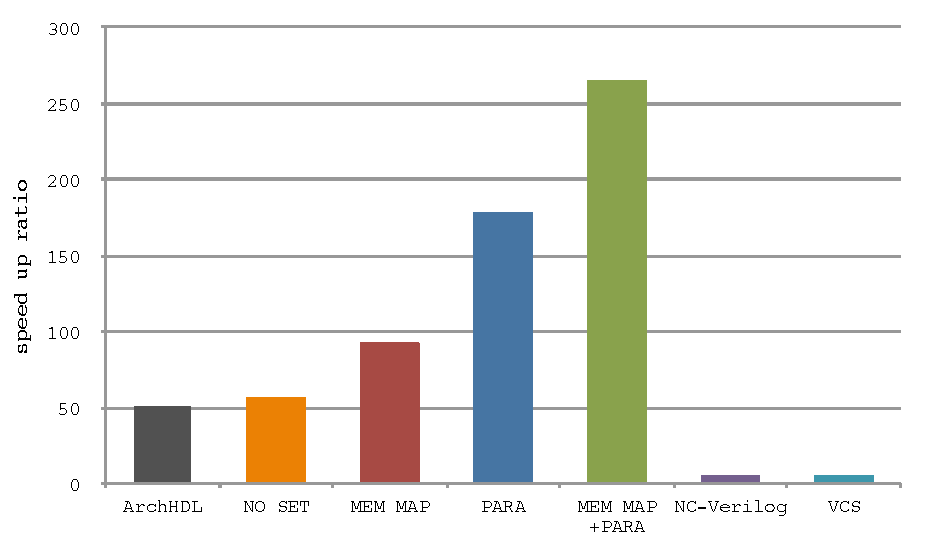
\includegraphics[clip,width=\linewidth]{counter_4096}
 \caption{4096 個のカウンター回路の実行時間の Icarus Verilog と比較した速度向上比}
 \label{fig:counter4096}
\end{figure}

\figref{fig:counter4096} に 4096 個のカウンター回路の実行時間の Icarus Verilog と比較した速度向上比を示す.
縦軸は Icarus Verilog での実行時間を 1 とした速度向上比を示している.

ArchHDL は商用の NC-Verilog, VCS と比較してもかなり高速である.
高速化手法と並列化を共に適用した場合と比べると ArchHDL は NC-Verilog の約 58.8 倍,VCS の約 56.7 倍高速である.

また今回提案している高速化手法は効果が出ている.
高速化手法と並列化を共に適用した ArchHDL のシミュレーションはオリジナルの ArchHDL より約 5.23 倍高速である.



\begin{figure}[t]
 \centering
 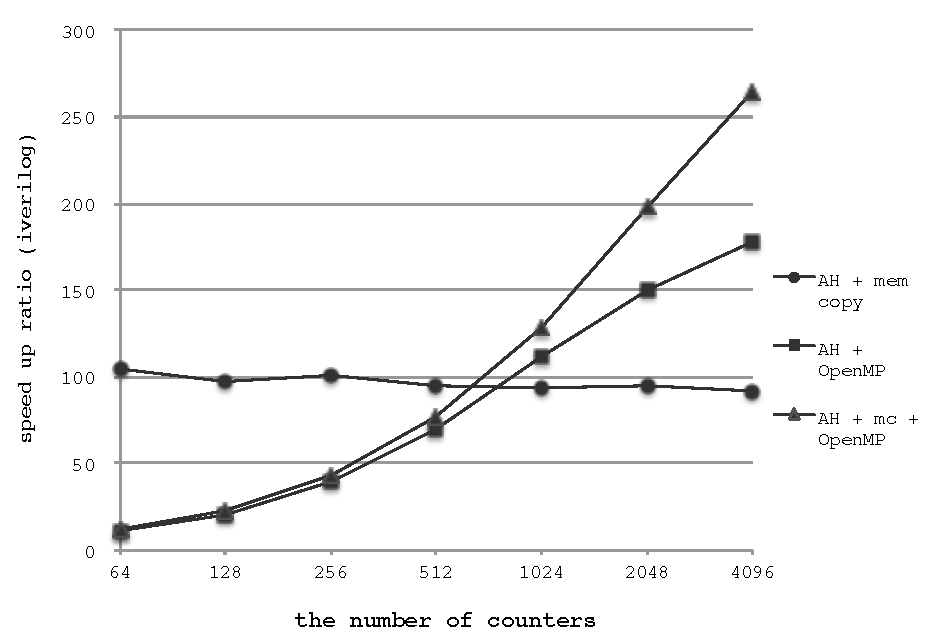
\includegraphics[clip,width=\linewidth]{counter_openmp}
 \caption{高速化手法を適用した ArchHDL と OpenMP を適用したカウンター回路の実行時間の Icarus Verilog と比較した速度向上比}
 \label{fig:counter_con}
\end{figure}

\figref{fig:counter_con} に高速化手法を適用した ArchHDL と OpenMP を適用したカウンター回路の実行時間の Icarus Verilog と比較した速度向上比を示す.
縦軸は Icarus Verilog での実行時間を 1 とした速度向上比を示している.
横軸はカウンターの個数である.

逐次実行は Icarus Verilog と比較して速度向上比はほぼ一定である.
並列化を行った場合はカウンターの個数が 1024 個を超えた所で逐次実行よりも高速になる.

カウンターの個数はハードウェアの規模とみなせるため,並列化が有効なのはある程度規模の大きい回路であると言える.

また \ref{sss:mem_copy} 節で述べた高速化手法は並列化を行った場合でも一貫して効果が出せている.

\begin{figure}[t]
 \centering
 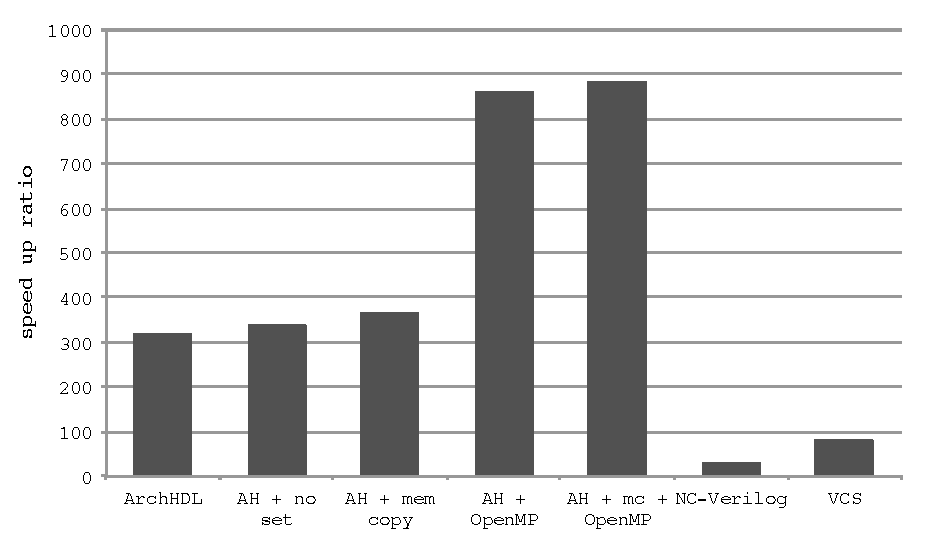
\includegraphics[clip,width=\linewidth]{xorshift}
 \caption{XORSHIFT による乱数生成器の実行時間の Icarus Verilog と比較した速度向上比}
 \label{fig:xorshift}
\end{figure}

\figref{fig:xorshift} は XORSHIFT による乱数生成器での実行時間の Icarus Verilog と比較した速度向上比である.
試行回数は 524,288 回である.初期値の異なる乱数生成器を 512 個用意している.

ArchHDL は商用の NC-Verilog, VCS と比較してもかなり高速である.
高速化手法と並列化を共に適用した場合と比べると ArchHDL は NC-Verilog の約 32.2 倍,VCS の約 11.3 倍高速である.

高速化手法と並列化を共に適用した ArchHDL のシミュレーションはオリジナルの ArchHDL より約 2.78 倍高速である.


\subsection{ステンシル計算回路による評価}

\if0

\begin{table}[t]
 \caption{ステンシル計算回路でのプロファイリング結果 1.1}
 \label{table:stencil_prof1.1}
 \begin{center}
  % \setlength{\tabcolsep}{3pt}
  \begin{tabular}{lr} \toprule
  関数名 & 実行時間に占める割合 (\%) \\ \midrule
  reg::Update() (合計) & 16.57 \\
  ArchHDL::Step() & 12.47 \\
  brk & 15.05 \\ \bottomrule
  \end{tabular}
 \end{center}
\end{table}

\fi

\begin{figure}[t]
 \centering
 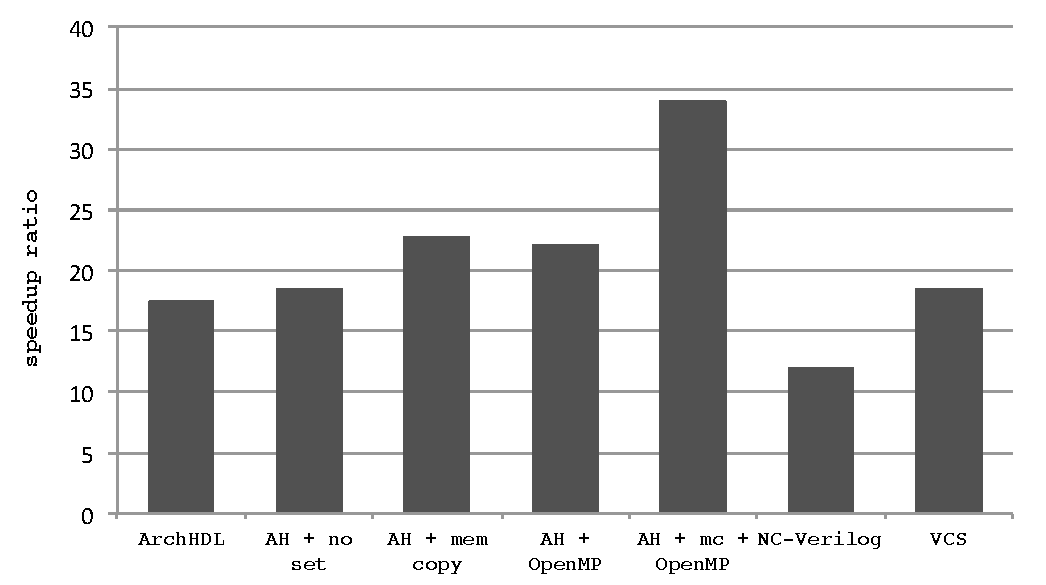
\includegraphics[clip,width=\linewidth]{stencil}
 \caption{ステンシル計算回路の Icarus Verilog と比較した実行時間の速度向上比}
 \label{fig:stencil}
\end{figure}

\figref{fig:stencil} はステンシル計算回路での実行結果である.

縦軸は Icarus Verilog と比較したそれぞれの速度向上比である.

OpenMP による並列化はスレッド数を 8 個にして計測している.

ステンシル計算回路の場合は Update() は 325,469,175 回呼ばれているのに対して,
reg の値が更新されるのは 320,323,415 回であり, reg の値に更新がないのは 5,145,760 回である.
つまり更新がないのは全体の約 $1.58\%$ 程度に過ぎない.
そのため \ref{sss:no_set} 節で述べたデータ変更の有無による条件分岐の除去を行った方が高速になる.

また Update() は 325,469,175 回呼ばれているのでこのメソッド呼び出しを減らし,
かつ代入をメモリーコピーにする \ref{sss:mem_copy} 節の逐次代入をメモリーコピーにする方が高速になっている.

また Module が 133 個,reg が 991 個存在する回路なので並列化の効果も大きい.

NC-Verilog は ArchHDL より高速でない.
VCS は ArchHDL と set\_ 変数なしの実装より高速であるが,メモリーコピーにする実装よりは高速でない.

高速化手法と並列化を共に適用した場合と比べると ArchHDL は VCS より約 1.83 倍高速である.




% \subsection{高速化の解析}
